
\tikzstyle{Absch} = [rectangle, draw, 
    text centered]
\tikzstyle{keinBeweis} = [rectangle, fill=gray!25, 
    text centered]    

\tikzstyle{BewTeil} = []


\tikzstyle{Box} = [rectangle, draw, text centered, rounded corners]
\tikzstyle{Alg} = [rectangle, draw, fill=gray!50, text centered]
\tikzstyle{Text} = [text centered]
\tikzstyle{Image} = []

\tikzstyle{arrow} = [draw, -latex']
\tikzstyle{line} = [draw]


\begin{tikzpicture}[node distance = 5em, auto]

% EINGABE:
\node [Box, text width=20em] (input) {\textbf{Input:} \\ \CLR-Instanz $((\ClientSet\cup\FacilitySet,E),c,\phi,d,u)$};
\node [below of=input] (under-input) {};
\node [Image, above of=input, node distance=6em] (input-img) {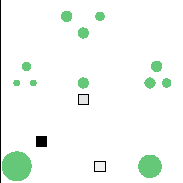
\includegraphics[width=8em]{bilder/instance.pdf}};

% UFL-Instanz:
\node [Box, left of=under-input, text width=15em, node distance=8.5em] (UFL) 
	{\textbf{UFL-Instanz:} \\ $((\ClientSet\cup\FacilitySet,E),\tilde{c},\phi,d)$ \\
	wobei $\tilde{c}:E \to \IR_{\geq 0}: e \mapsto \frac{2}{u}c(e)$};
\node [Text, left of=UFL, text width=12em, node distance=17em] (UFL-lower-bound) {$\leadsto$ Untere Schranke: $\text{\OPT}(\text{\CLR}) \geq \text{\OPT}(\text{\UFL})$};
\node [Alg, below of=UFL, text width=15em] (UFL-solving) {löse approximativ (mit Greedy)};
\node [Image, left of=UFL-solving, node distance=16.5em] (UFL-img) {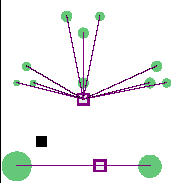
\includegraphics[width=5em]{bilder/UFL.pdf}};

% MST-Instanz:
\node [Box, right of=under-input, text width=15em, node distance=8.5em] (MST)
	{\textbf{\MST-Instanz:} \\ $((\ClientSet\cup\FacilitySet\cup\{r\},E^\prime),c^\prime)$ \\
	$E^\prime := E \cup \{\{r,f\}\mid f\in\FacilitySet\}$ \\
	$c^\prime(f,v) := c(f,v) + \frac{1}{2}\phi(f),$ \\
	$c^\prime(r,f) := 0, c^\prime(v,w):=c(c,w)$};
\node [Text, right of=MST, text width=12em, node distance=17em] (MST-lower-bound) {$\leadsto$ Untere Schranke: $\text{\OPT}(\text{\CLR}) \geq \text{\OPT}(\text{\MST})$};
\node [Alg, below of=MST, text width=15em] (MST-solving) {löse exakt $\leadsto$ Spannbaum $B$};
\node [Image, right of=MST-solving, node distance=17em] (MST-img) {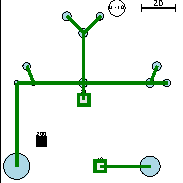
\includegraphics[width=5em]{bilder/MST.pdf}};

% MERGE-Phase:
\node [Text, below of=under-input, node distance=8em] (merge) {\textbf{Merge-Phase:}};

\node [Alg, below of=merge, node distance=1.5em, text width=32em] (m-facilities) {
		\begin{minipage}{30em}\begin{algorithmic}
		\State Eröffne in \UFL{} oder \MST{} verwendete Fabriken
		\end{algorithmic}\end{minipage}
	};
\node [Text, left of=m-facilities, node distance=25em, text width=15em] () 
	{Kosten beschränkt durch die entsprechenden Eröffnungskosten in \UFL{} und \MST{}};

% Große Kunden
\node [Alg, below of=m-facilities, node distance=4em] (m-big-clients) {
		\begin{minipage}{32em}\begin{algorithmic}
		\For{Kunden $v$ mit $d(v)\geq u$}
			\State Verbinde $v$ durch $\ceil{\frac{d(v)}{u}}$ Touren mit nächster offener Fabrik
		\EndFor
		\end{algorithmic}\end{minipage}
	};
\node [Image, right of=m-big-clients, node distance=25em] () {
	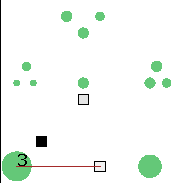
\includegraphics[width=5em]{bilder/largeDemand1.pdf}
	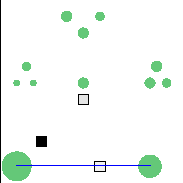
\includegraphics[width=5em]{bilder/largeDemand2.pdf}
};
\node [Text, left of=m-big-clients, node distance=25em, text width=15em] () 
	{Kosten beschränkt durch $2\times$ den entsprechenden Verbindungskosten in \UFL};

% Kleine Kunden
\node [Alg, below of=m-big-clients, node distance=5em] (m-small-clients) {
		\begin{minipage}{32em}\begin{algorithmic}\algtext*{EndFor}
		\For{durch \MST{} eröffnete Fabrik $f$}
		\State Betrachte $B$ als gerichteten Baum mit Wurzel $r$
		\State Für Knoten $v$ ist $B_v$ der Teilbaum mit Wurzel $v$
		\EndFor
		\end{algorithmic}\end{minipage}
	};

% Relieve-Schritte
\node [Alg, below of=m-small-clients, node distance=7em] (m-relieve) {
		\begin{minipage}{32em}\begin{algorithmic}\algtext*{For}\algtext*{EndFor}
			\For
			\While{$d(B_f) > 0$}
			\State Sei $v \in B_f: d(B_v) > u$ und $d(B_w) \leq u$ f.a. Kinder $w$ von $v$
			\State Partitioniere die Menge der Unterbäume von $B_v$ 
			\State \quad in Mengen mit Bedarf zw. $u/2$ und $u$
			\State Wandle diese zu Touren um und verbinde sie jeweils
			\State \quad mit nächster offener Fabrik
			\EndWhile
			\EndFor
			\end{algorithmic}\end{minipage}
	};
\node [Image, right of=m-relieve, node distance=25em] () {
		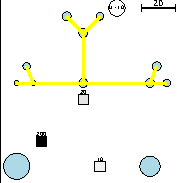
\includegraphics[width=5em]{bilder/relieveTour1.pdf}
		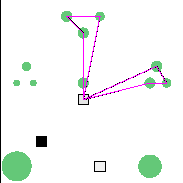
\includegraphics[width=5em]{bilder/relieveTour2.pdf}
		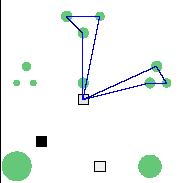
\includegraphics[width=5em]{bilder/relieveTour3.pdf}
	};
\node [Text, left of=m-relieve, node distance=25em, text width=15em] () 
	{Kosten beschränkt durch $2\times$ die Kantenkosten im \MST{} und $2\times$ den Verbindungskosten aller Knoten der Tour in \UFL};

% Rest
\node [Alg, below of=m-relieve, node distance=7em] (m-remaining) {
		\begin{minipage}{32em}\begin{algorithmic}\algtext*{For}
		\For
		\State Übrige Kunden in $B_f$ (mit Gesamtbedarf $\leq u$) zu Tour verbinden 
		\State und mit nächster offener Fabrik verbinden
		\EndFor
		\end{algorithmic}\end{minipage}
	};
\node [Image, right of=m-remaining, node distance=25em] () {
	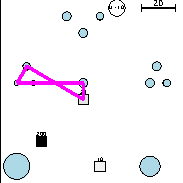
\includegraphics[width=5em]{bilder/remainingTour1.pdf}
	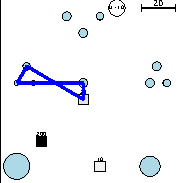
\includegraphics[width=5em]{bilder/remainingTour2.pdf}
};
\node [Text, left of=m-remaining, node distance=25em, text width=15em] () 
	{Kosten beschränkt durch $2\times$ den Verbindungskosten in \MST};


% AUSGABE:
\node [Box, below of=m-remaining, node distance=4em] (output) {\textbf{Output:} offene Fabriken $F$ und Touren $\Tc$};
\node [Image, below of=output] (outpu-img) {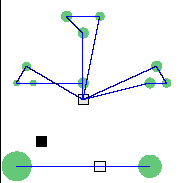
\includegraphics[width=8em]{bilder/output.pdf}};


% PATHS:

\path [arrow] (input.south) -- (UFL.north);    
\path [arrow] (input.south) -- (MST.north); 

\path [arrow] (UFL) -- (UFL-solving.north);
\path [arrow] (MST) -- (MST-solving.north);
\path [arrow] (UFL-solving.south) -- (merge.north);
\path [arrow] (MST-solving.south) -- (merge.north);

\path [line] (m-facilities) -- (m-big-clients);
\path [line] (m-big-clients) -- (m-small-clients);
\path [line] (m-small-clients) -- (m-relieve);
\path [line] (m-relieve) -- (m-remaining);

\path [arrow] (m-remaining.south) -- (output.north);

\end{tikzpicture}
